\subsection{Atacar un territorio}

\begin{figure}[ht]
\centering
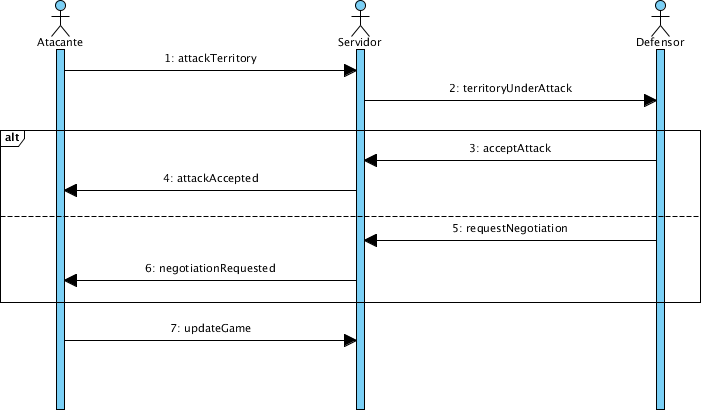
\includegraphics[scale=0.6]{img/ch03devel-attack.png}
\caption{Flujo de acciones de ``Atacar un territorio''}
\end{figure}

Una vez iniciada una partida, el jugador puede realizar un determinado número de
acciones, entre las que se incluye atacar otro territorio. Esta acción se
compone de una serie de subacciones que se deben realizar en coordinación con
el cliente defensor, usando el servidor como intermediario.

De este caso de uso se han creado cuatro diagramas de secuencia, los cuales son
demasiado extensos para ser mostrados en esta memoria. Por este motivo, se
remite al lector al proyecto de Visual Paradigm aportado.

Desde el punto de vista del atacante, al jugador se le muestra una ventana
diálogo donde deberá indicar la cantidad de unidades con las que desee atacar.
El motor del juego creará con estos datos un objeto de tipo \texttt{Attack}, y
realizará la petición de ataque al servidor.

Pasa un tiempo, el servidor realizará una de estas dos llamadas:
\texttt{attackAccepted} o \texttt{negotiationRequested}. En el caso de la
primera opción, el motor del juego resolverá el ataque y actualizará el
servidor con los datos después del combate, eliminando además el objeto
\texttt{Attack}.

En el caso de que se haya solicitado una negociación, se almacenará las
cantidades de soldados y gallifantes ofrecidos y se comunicará a la ventana
principal del evento ocurrido. Ésta mostrará al usuario un mensaje en el que
deberá elegir si desea negociar o no. Según su respuesta, el motor del juego
resolverá la situación y actualizará el servidor.

Desde el punto de vista del defensor, la acción comienza con la recepción del
mensaje \texttt{territoryUnderAttack}. El motor del juego notifica entonces a
la ventana principal, la cual presenta al usuario la decisión de aceptar el
ataque o negociar. En función de la respuesta del usuario, se realizará una
llamada u otra.